% Provenance (never printed): see sources/outline_sources.md (Year 3: the main
% field and its secular variation, rock magnetism, palaeomagnetic poles, apparent
% polar wander, magnetostratigraphy, the geodynamo). Brief: sources/book5/BRIEFS.md,
% ch. 4. Curves and maps from figdata/bachelor-3/igrf_field.py (IGRF-14),
% palaeomag_stats.py (the invented Kesta terrane, its Fisher statistics, the
% Zijderveld specimen and the reference APW path), magnetostratigraphy.py.
% Exercise and problem values in the Book 5 scratch calculator calc/ch04.py.
\chapter{地磁学与古地磁学}\label{ch:b3:palaeomagnetism}

一块在 6000 万年前喷发并冷却的玄武岩流，其中细小的磁铁矿颗粒
按当时的磁场方向定向排列并被锁定。今天将其原位定向钻取，
切割成小圆柱体，并在屏蔽了当前磁场的房间中逐步加热，
它仍能说明当时它距极点有多远，
以及当时它朝向哪个方向。成千上万次此类测量遍及各大陆、各个时代，
已说明大陆如何在记录其运动的洋底诞生之前发生移动，
以及地磁场在沉积剖面各层中按怎样的顺序发生倒转。
本章将介绍地磁场今天的状态，
岩石如何记录地磁场，如何提取并平均方向，
以及古地磁极能说明板块运动的
哪些信息。

\begin{recall}
地球作为磁体以及磁偏角，见物理学各册的中学分册；
磁畴、磁滞、剩磁以及居里温度，见其本科三年级分册；
磁偶极子的场，见其本科一年级分册。
地磁倒转以及正、反极性，在十一年级时已接触过。
大圆与球面三角形在本科一年级分册的球面天文一章中已定义；
极性时、地磁极性年表、海洋磁异常以及绕欧拉极的有限旋转，
见其板块运动球面几何一章；热点轨迹见其热点一章。
球谐函数以及施密特归一化的勒让德函数 $P_n^m$
曾在关于重力与地球形状的一章
（\cref{ch:b3:gravity-geodesy}）
中用于重力计算。
\end{recall}

\section{主磁场}

\begin{definition}[地磁主磁场；地心轴向偶极子]\label{def:b3:palaeomagnetism:main-field}
\emph{地磁主磁场}\index{地磁主磁场}是地球磁场中产生于地球内部的部分，
源于液态铁质外核；其变化时间尺度从数年到数百万年不等，
与之不同，电离层与磁层的场
则在数秒到数天之间变化。
\emph{地心轴向偶极子}\index{地心轴向偶极子}是放置在地心、与自转轴对齐的
磁偶极子所产生的场，其方向指向南方，
因此其磁场线从南半球射出，
并进入北半球。
\end{definition}

地表任一点的磁场 $\mathbf F$ 是一个矢量。在局部坐标系中（见下图）描述它：
$X$ 指向地理北，$Y$ 指向东，
$Z$ 指向下方。其水平分量为 $H = \sqrt{X^2 + Y^2}$，
总强度为 $F = |\mathbf F|$，磁偏角 $D$ 为从地理北到
$\mathbf H$ 的顺时针夹角，其\omterm{def:b3:palaeomagnetism:inclination}{磁倾角} $I$ 为
从水平面到 $\mathbf F$ 的夹角。

\begin{definition}[磁倾角]\label{def:b3:palaeomagnetism:inclination}
某点处磁场的\emph{磁倾角}\index{磁倾角} $I$ 是
该点磁场矢量与水平面之间的夹角，
磁场指向下方时取正值：$\tan I = Z/H$，且 $-\ang{90} \le I
\le \ang{90}$。
\end{definition}

\begin{omfigure}
\begin{tikzpicture}[font=\small, x=1cm, y=1cm, >={Stealth[length=5pt]}]
% schematic; X = 3.0, Y = 1.0 (along the oblique east axis), Z = 2.4
\coordinate (O) at (0,0);
\coordinate (E) at (0.9,0.65);
\fill[gray!12] (-0.6,-0.43) -- (3.6,-0.43) -- ($(3.6,-0.43)+2.2*(E)$) -- ($(-0.6,-0.43)+2.2*(E)$) -- cycle;
\draw[->] (O) -- (4.0,0) node[right] {$X$，地理北};
\draw[->] (O) -- ($1.9*(E)$) node[above right] {$Y$，东};
\draw[->] (O) -- (0,-3.0) node[below] {$Z$，向下};
\coordinate (Hh) at ($(3.0,0)+1.0*(E)$);
\coordinate (F) at ($(Hh)+(0,-2.4)$);
\draw[densely dashed, gray] (3.0,0) -- (Hh);
\draw[densely dashed, gray] ($1.0*(E)$) -- (Hh);
\draw[densely dashed, gray] (Hh) -- (F);
\draw[densely dashed, gray] (0,-2.4) -- (F);
\draw[very thick, ->, blue!60!black] (O) -- (Hh) node[pos=0.3, above, sloped] {$\mathbf H$};
\draw[very thick, ->, red!70!black] (O) -- (F) node[pos=0.55, below left] {$\mathbf F$};
\draw[thick] (1.25,0) arc[start angle=0, end angle=9.46, radius=1.25];
\node at (1.62,0.13) {$D$};
\draw[thick, red!70!black] ($0.36*(Hh)$) to[bend left=30] ($0.3*(F)$);
\node[red!70!black] at (1.62,-0.42) {$I$};
\end{tikzpicture}

\par\smallskip{\small 地表某点磁场的各要素：北向分量 $X$、东向
分量 $Y$ 与向下分量 $Z$、水平分量 $\mathbf H$、总场
$\mathbf F$、磁偏角 $D$（位于水平面内，灰色区域）
以及\omterm{def:b3:palaeomagnetism:inclination}{磁倾角} $I$（位于包含 $\mathbf
F$ 的竖直面内）。}\label{fig:b3:palaeomagnetism:elements}
\end{omfigure}

\begin{theorem}[偶极子公式]\label{thm:b3:palaeomagnetism:dipole}
在半径为 $a$ 的球面上，磁矩为 $m$ 的\omterm{def:b3:palaeomagnetism:main-field}{地心轴向偶极子}场
在纬度 $\lambda$ 处为
\[
  H = B_0\cos\lambda,\qquad Z = 2B_0\sin\lambda,\qquad
  F = B_0\sqrt{1 + 3\sin^2\lambda},\qquad
  \tan I = 2\tan\lambda,\qquad D = 0,
\]
其中 $B_0 = \mu_0 m/(4\pi a^3)$ 为赤道处的场强。这就是
\emph{偶极子公式}\index{偶极子公式}。
\end{theorem}

\begin{proof}
在源之外，磁场由磁标势导出，
$\mathbf B = -\nabla V$。对于磁矩为 $m$、指向 $-z$ 的偶极子，
即地理南方，$V = -\mu_0 m\cos\theta/(4\pi r^2)$，其中 $\theta$ 为
余纬。在球坐标中，$B_r = -\partial V/\partial r =
-2\mu_0 m\cos\theta/(4\pi r^3)$ 和 $B_\theta = -(1/r)\,\partial V/\partial\theta =
-\mu_0 m\sin\theta/(4\pi r^3)$，且 $B_\varphi = 0$。在 $r = a$ 处，向下分量
为 $Z = -B_r = 2B_0\cos\theta = 2B_0\sin\lambda$，由于
$\mathbf e_\theta$ 指向南方，指向北方的分量为 $X = -B_\theta =
B_0\sin\theta = B_0\cos\lambda$，且 $Y = 0$。于是 $H = X$，$D = 0$，$\tan I =
Z/H = 2\tan\lambda$，并且 $F^2 = B_0^2(\cos^2\lambda + 4\sin^2\lambda) =
B_0^2(1 + 3\sin^2\lambda)$。
\end{proof}

赤道处的倾角为零，北极处为 \ang{90}，
南半球的倾角为负值；两极处的强度
是赤道处的两倍。实际磁场并非完美的偶极子，它与重力一样，
用球谐函数来描述。

\begin{definition}[国际地磁参考场]\label{def:b3:palaeomagnetism:igrf}
\emph{国际地磁参考场}\index{国际地磁参考场}
（IGRF）是国际公认的主磁场模型，即
地表上及地表之上的势：
\[
  V(r,\theta,\varphi) = a\sum_{n=1}^{N}\Bigl(\frac ar\Bigr)^{n+1}\sum_{m=0}^{n}
  \bigl(g_n^m\cos m\varphi + h_n^m\sin m\varphi\bigr)P_n^m(\cos\theta),
\]
其中 $a = \qty{6371.2}{km}$，$\mathbf B = -\nabla V$，高斯系数
$g_n^m$、$h_n^m$（单位为 \unit{nT}）自 1900 年起每五年给出一次，并
附有其后五年的变化率。
\end{definition}
% ledger: geomag5:igrf, data:b5-igrf

该模型由国际地磁与高层大气协会维护，第十四代模型于
2024 年 11 月完成，截断至
$N = 13$ 阶。第一项 $g_1^0$ 为轴向偶极子：
对照上文的证明，$B_0 = -g_1^0$，且 $g_1^0 = \qty{-29350}{nT}$（2025 年）。
加上另外两个一阶项后，偶极子发生倾斜，其轴与
地表相交于北地磁极，该点于 2025 年位于北纬 \ang{80.79}，西经 \ang{72.76}，
其磁矩为 $m = 4\pi a^3\sqrt{(g_1^0)^2 + (g_1^1)^2 +
(h_1^1)^2}/\mu_0 = \qty{7.69e22}{A.m^2}$。
% ledger: data:b5-igrf

\begin{omfigure}
\begin{tikzpicture}
\begin{groupplot}[group style={group size=1 by 2, vertical sep=1.4cm},
  ommap, width=0.96\linewidth, xtick={-180,-120,...,180}, ytick={-60,0,60},
  unbounded coords=jump, title style={font=\small, yshift=-1ex}]
\nextgroupplot[title={(a) 倾角，每 \ang{20}}]
% computed in figdata/bachelor-3/igrf_field.py; ledger: data:b5-igrf, data:ne-land
\addplot[fill=omLithAlluv, draw=black!45, line width=0.2pt, forget plot] table {figdata/out/shared-geo-land.dat};
\addplot[red!70!black, line width=0.5pt] table[x=x, y=y] {figdata/out/bachelor-3-igrf_field-incl.dat};
\addplot[black, line width=1.1pt] table[x=x, y=y] {figdata/out/bachelor-3-igrf_field-dipeq.dat};
\addplot[draw=none, nodes near coords, point meta=explicit,
  every node near coord/.style={font=\tiny, fill=white, inner sep=0.6pt, anchor=center}]
  table[x=x, y=y, meta=lev] {figdata/out/bachelor-3-igrf_field-inclab.dat};
\nextgroupplot[title={(b) 总强度，每 \qty{5000}{nT}}]
\addplot[fill=omLithAlluv, draw=black!45, line width=0.2pt, forget plot] table {figdata/out/shared-geo-land.dat};
\addplot[blue!60!black, line width=0.5pt] table[x=x, y=y] {figdata/out/bachelor-3-igrf_field-intens.dat};
\addplot[draw=none, nodes near coords, point meta=explicit,
  every node near coord/.style={font=\tiny, fill=white, inner sep=0.6pt, anchor=center}]
  table[x=x, y=y, meta=lev] {figdata/out/bachelor-3-igrf_field-intlab.dat};
\addplot[only marks, mark=x, mark size=3pt, line width=1pt, black] table {figdata/out/bachelor-3-igrf_field-fmin.dat};
\end{groupplot}
\end{tikzpicture}

\par\smallskip{\small 2025 年的主磁场，取自第十四代 IGRF，位于
半径为 \qty{6371.2}{km} 的球面地表。（a）倾角，单位为度；
粗线 $I = 0$ 为倾角零线。（b）总强度，单位为 \unit{nT}；
十字标记最弱的磁场，约 \qty{22100}{nT}，位于南
大西洋上空；最强处约 \qty{66600}{nT}，位于
澳大利亚以南。}\label{fig:b3:palaeomagnetism:igrf-maps}
\end{omfigure}

上图显示了磁场偏离偶极子的程度。倾角零线
与地理赤道的偏离最大约 \ang{12}，而强度
在偶极子模型下沿纬线处处相等，实际却相差
约三倍，南大西洋上空有一片宽广的低值区。
% ledger: data:b5-igrf

\begin{definition}[长期变化]\label{def:b3:palaeomagnetism:secular}
\emph{长期变化}\index{长期变化}是主磁场
随时间的缓慢变化，时间尺度为数年至数世纪，
通过高斯系数或某地磁场要素的变化率来度量。
\end{definition}

过去 125 年间，偶极矩由
\qty{8.32e22}{A.m^2} 降至 \qty{7.69e22}{A.m^2}，减少了 \qty{7.6}{\percent}，
北地磁极由北纬 \ang{78.61}、西经 \ang{68.79} 移至其
现在的位置（见下图）；$g_1^0$ 仍以每年 \qty{12.6}{nT} 的速度增长，
表明偶极子在减弱。
% ledger: data:b5-igrf

\begin{omfigure}
\begin{tikzpicture}
\begin{groupplot}[group style={group size=2 by 1, horizontal sep=1.7cm},
  omrecord, width=0.47\linewidth, height=0.4\linewidth, xmin=1895, xmax=2030,
  xtick={1900,1950,2000}, xticklabel style={/pgf/number format/1000 sep=},
  xlabel={年份}]
\nextgroupplot[ylabel={偶极矩（\qty{e22}{A.m^2}）}, ymin=7.6, ymax=8.4]
% computed in figdata/bachelor-3/igrf_field.py; ledger: data:b5-igrf
\addplot[omDef, thick, mark=*, mark size=1pt] table[x=year, y=M] {figdata/out/bachelor-3-igrf_field-dipole.dat};
\nextgroupplot[ylabel={北地磁极纬度（\unit{\degree}\,北）}, ymin=78, ymax=81.5]
\addplot[red!70!black, thick, mark=*, mark size=1pt] table[x=year, y=plat] {figdata/out/bachelor-3-igrf_field-dipole.dat};
\end{groupplot}
\end{tikzpicture}

\par\smallskip{\small 1900--2025 年主磁场中的偶极子部分，每五年一个数据点，
取自 IGRF，左图为其偶极矩，
右图为北地磁极的纬度。}\label{fig:b3:palaeomagnetism:dipole}
\end{omfigure}

地磁场从何而来？永久磁铁已被排除：磁铁矿的居里
温度约为 \qty{580}{\celsius}，赤铁矿约为
\qty{675}{\celsius}，地球深部远比此炽热。磁场
是由导电液体的运动持续再生的，这些液体位于
外核中。
% ledger: tarduno:curie

\begin{definition}[地球发电机]\label{def:b3:palaeomagnetism:geodynamo}
\emph{地球发电机}\index{地球发电机}是一种自我维持的过程：
外核中导电的液态铁合金因对流，
受地球自转偏转，感生出电流，电流产生的磁场
克服欧姆耗散而维持自身。
\end{definition}

\begin{proposition}[感应方程]\label{prop:b3:palaeomagnetism:induction}
设磁扩散率为 $\eta = 1/(\mu_0\sigma)$ 的导体以
速度 $\mathbf u$ 运动，则磁场满足
\[
  \frac{\partial\mathbf B}{\partial t} = \nabla\times(\mathbf u\times\mathbf B)
  + \eta\nabla^2\mathbf B .
\]
\end{proposition}
\admitted

第一项拉伸并扭转由流动携带的场线；
第二项使磁场衰减，在尺度为 $L$ 的物体中，衰减时间的量级为
$L^2/\eta$。当流动再生磁场的速度快于磁场向外扩散时，发电机即能工作。
对对流、旋转的流体壳层进行计算机模拟，
能够再现占主导的轴向偶极子，并时而出现倒转；
但\omterm{def:b3:palaeomagnetism:geodynamo}{地球发电机}的方程及其与流动方程的耦合超出了本书的范围。
除完全倒转外，古地磁记录中还保存有较短的事件。

\begin{definition}[地磁漂移]\label{def:b3:palaeomagnetism:excursion}
\emph{地磁漂移}\index{地磁漂移}是指磁场方向
与轴向偶极子方向发生较大偏离，
\omterm{def:b3:palaeomagnetism:vgp}{虚地磁极}（见\cref{def:b3:palaeomagnetism:vgp}）远离地理极，
随后磁场回到原来的极性，
而不完成倒转。
\end{definition}

\section{岩石如何记录磁场}

广义上的铁磁性矿物，主要是火成岩中的磁铁矿与红色沉积物中的赤铁矿，
它们携带剩磁。高于居里温度时，颗粒没有剩磁；
低于居里温度时，小颗粒是单一磁畴，其磁矩在易磁化方向之间翻转，
翻转是热激活过程，所需的
弛豫时间为
\[
  \tau = \frac1C\exp\Bigl(\frac{K V}{k_B T}\Bigr),
\]
其中 $K$ 为单位体积的各向异性能，$V$ 为颗粒的体积，
$C$ 为频率因子。这是奈尔弛豫定律，在本阶段不加证明地承认。由于
$\tau$ 随 $T$ 降低呈指数增长，颗粒在很窄的温度区间内，
从自由翻转转变为能将磁矩保持数十亿
年。

\begin{definition}[阻挡温度]\label{def:b3:palaeomagnetism:blocking}
磁性颗粒的\emph{阻挡温度}\index{阻挡温度}是指
这样一个温度：低于它时，颗粒的弛豫时间超过实验时间，
磁矩保持固定。冷却经过该温度时，颗粒记录下磁场；
在零场中加热经过该温度时，颗粒
失去这一记录。
\end{definition}

\begin{definition}[天然剩磁、热剩磁、碎屑剩磁与化学剩磁]\label{def:b3:palaeomagnetism:nrm}
岩石的\emph{天然剩磁}\index{天然剩磁}（NRM）是指岩石
在采集时所携带的剩磁，它是在不同时间获得的
各分量之和。\emph{热剩磁}\index{热剩磁}（TRM）是在磁场中
冷却经过\omterm{def:b3:palaeomagnetism:blocking}{阻挡温度}时获得的，
例如熔岩流或侵入体。
\emph{碎屑剩磁}\index{碎屑剩磁}（DRM）是
磁性颗粒在水中沉降，或在紧贴其表面的湿沉积物中沉降时，
在被锁定之前转向磁场而获得的。
\emph{化学剩磁}\index{化学剩磁}（CRM）是磁性矿物
在磁场中生长、穿过阻挡体积时获得的，
例如红层形成时赤铁矿的生成。
\end{definition}

TRM 记录的是冷却时刻的磁场；DRM 记录的是沉积物压实
所需时间内的磁场；CRM 则记录矿物生长时的磁场，
这可能远在沉积之后。之后的加热，或当前磁场长时间作用于
弛豫时间较短的颗粒，会在其上叠加一个次生分量：
沿当前磁场方向的粘滞剩磁。

\section{从样品到方向}

在一个地层中的若干地点钻取定向岩芯，每个地点取若干根，
再切割成体积为几立方厘米的样品。先测量每个样品的\omterm{def:b3:palaeomagnetism:nrm}{天然剩磁}，
然后逐步将其去除。

\begin{definition}[逐步退磁]\label{def:b3:palaeomagnetism:demag}
\emph{逐步退磁}\index{逐步退磁}是指
以递增强度逐级去除样品的剩磁，并在每一级之后测量
剩余矢量：一是逐级升温加热，再在零场中冷却
（热退磁），先去除\omterm{def:b3:palaeomagnetism:blocking}{阻挡温度}较低的
分量；二是施加峰值递增、再衰减至零的交变磁场
（交变场退磁），先去除
矫顽力较低的分量。
\end{definition}

\begin{definition}[Zijderveld 图；特征剩磁]\label{def:b3:palaeomagnetism:zijderveld}
\emph{Zijderveld 图}\index{Zijderveld 图}同时在两个平面上绘出每一级退磁后
剩余剩磁矢量的端点，两个平面分别为水平面（北对东）
与竖直面（北对下），
两者共用北向坐标轴。单独去除的一个分量，在一系列退磁级上
呈直线段；终止于原点的线段即为
\emph{特征剩磁}\index{特征剩磁}（ChRM），
它是最稳定的分量，在检验允许时
被解释为原生剩磁。
\end{definition}

下图中的样品携带两个分量：一是沿当前磁场的粘滞叠加分量，
在 \qty{300}{\celsius} 时被去除；二是\omterm{def:b3:palaeomagnetism:zijderveld}{特征剩磁}（ChRM），
在 300 至 \qty{580}{\celsius} 之间解阻，\qty{580}{\celsius} 为磁铁矿的居里温度。
高于 \qty{300}{\celsius} 时，两个投影都直线指向原点；
该线段的方向即为\omterm{def:b3:palaeomagnetism:zijderveld}{特征剩磁}的方向。

\begin{omfigure}
\begin{tikzpicture}
\begin{groupplot}[group style={group size=2 by 1, horizontal sep=1.3cm},
  width=0.5\linewidth]
\nextgroupplot[axis lines=middle, axis equal image, xmin=-4, xmax=36, ymin=-4, ymax=42,
  y dir=reverse, xlabel={北}, ylabel={东，下}, tick label style={font=\scriptsize},
  xtick={0,10,20,30}, ytick={10,20,30,40}, label style={font=\small},
  xlabel style={at={(ticklabel* cs:1.0)}, anchor=west},
  ylabel style={at={(ticklabel* cs:1.0)}, anchor=north west},
  title={(a) Zijderveld 图（\unit{mA/m}）}, title style={font=\small, yshift=1ex},
  clip=false, legend style={font=\scriptsize, at={(0.13,0.03)}, anchor=south west, cells={anchor=west}}]
% computed in figdata/bachelor-3/palaeomag_stats.py (synthetic specimen)
\addplot[black, mark=*, mark size=1.5pt] table[x=N, y=E] {figdata/out/bachelor-3-palaeomag_stats-zij.dat};
\addlegendentry{水平面：北、东}
\addplot[black, mark=o, mark size=1.7pt, fill=white] table[x=N, y=Down] {figdata/out/bachelor-3-palaeomag_stats-zij.dat};
\addlegendentry{竖直面：北、下}
\node[font=\scriptsize, anchor=south west] at (axis cs:32.2,18.1) {\qty{20}{\celsius}};
\node[font=\scriptsize, anchor=north west] at (axis cs:32.2,38.2) {\qty{20}{\celsius}};
\node[font=\scriptsize, anchor=south] at (axis cs:25.8,17.6) {300};
\node[font=\scriptsize, anchor=east] at (axis cs:25.0,24.6) {300};
\node[font=\scriptsize, anchor=south east] at (axis cs:-0.5,-0.5) {580};
\nextgroupplot[axis equal image, hide axis, clip=false, xmin=-1.12, xmax=1.12, ymin=-1.12, ymax=1.18,
  title={(b) 地点 A，等面积投影，下半球}, title style={font=\small, yshift=1ex}]
\addplot[black, domain=0:360, samples=145, thin] ({cos(x)},{sin(x)});
\draw[black] (axis cs:0,1) -- (axis cs:0,1.08) node[above, font=\scriptsize] {北};
\draw[black] (axis cs:1,0) -- (axis cs:1.06,0);
\draw[black] (axis cs:0,-1) -- (axis cs:0,-1.06);
\draw[black] (axis cs:-1,0) -- (axis cs:-1.06,0);
\draw[black] (axis cs:-0.04,0) -- (axis cs:0.04,0) (axis cs:0,-0.04) -- (axis cs:0,0.04);
\addplot[only marks, mark=*, mark size=1.6pt, black] table[x=x, y=y] {figdata/out/bachelor-3-palaeomag_stats-dirsA.dat};
\addplot[omDef, thick] table[x=x, y=y] {figdata/out/bachelor-3-palaeomag_stats-cone.dat};
\addplot[only marks, mark=star, mark size=3.5pt, omDef, line width=0.9pt] table[x=x, y=y] {figdata/out/bachelor-3-palaeomag_stats-meanA.dat};
\end{groupplot}
\end{tikzpicture}

\par\smallskip{\small (a) 合成样品的热退磁，温度自
\qty{20}{\celsius} 至 \qty{580}{\celsius}：实心点为水平
分量投影；空心点为竖直分量投影。(b) 周末问题中站点 A 的六个 ChRM 方向（圆点）、
其平均方向（星形）及其 95\% 置信锥
（圆圈）。}\label{fig:b3:palaeomagnetism:zijderveld}
\end{omfigure}

同一采样点各样品的方向围绕某一平均方向散布，
这种散布的统计规律即球面上某一分布的规律。

\begin{proposition}[费希尔分布]\label{prop:b3:palaeomagnetism:fisher}
\emph{费希尔分布}\index{费希尔分布}（以某一平均方向为中心，精度参数 $\kappa > 0$）
给出单位矢量的
概率密度（按单位立体角计）：
\[
  f(\theta) = \frac{\kappa}{4\pi\sinh\kappa}\,e^{\kappa\cos\theta},
\]
其中 $\theta$ 为该矢量与平均方向的夹角。设自其中抽取 $N$ 个单位矢量 $\mathbf u_i$，
合矢量 $\mathbf R = \sum\mathbf u_i$ 的长度为 $R$，则
平均方向的最佳估计为 $\mathbf R$ 的方向；精度
由 $k = (N - 1)/(N - R)$ 估计；真实平均方向以概率
$1 - p$ 落在估计平均方向的夹角 $\alpha_{1-p}$ 之内，其中
\[
  \cos\alpha_{1-p} = 1 - \frac{N - R}{R}\Bigl[\Bigl(\frac1p\Bigr)^{1/(N-1)} - 1\Bigr].
\]
\end{proposition}
\admitted

\begin{definition}[alpha-95]\label{def:b3:palaeomagnetism:a95}
某一平均方向的 \emph{alpha-95}\index{alpha-95}（$\alpha_{95}$）是其
95\% 置信锥的半顶角，
即 $\alpha_{1-p}$（见\cref{prop:b3:palaeomagnetism:fisher}）中 $p = 0.05$ 时的角。
\end{definition}

密度积分为一：取 $\mathrm d\Omega = 2\pi\sin\theta\,\mathrm
d\theta$，则 $\int_0^\pi f\,2\pi\sin\theta\,\mathrm d\theta =
\frac{\kappa}{2\sinh\kappa}\cdot\frac{e^\kappa - e^{-\kappa}}{\kappa} = 1$。方向应作为单位矢量求平均，
而不能按角度求平均：偏角 \ang{350} 与 \ang{10} 的平均
为北向，而非南向。$k$ 越大，说明方向越集中，$\alpha_{95}$ 大致
以 $1/\sqrt{kN}$ 的规律减小。

\begin{method}[古地磁方向的野外检验]\label{met:b3:palaeomagnetism:tests}
ChRM 可借野外检验表明其形成早于某一事件。
\begin{itemize}
  \item \textbf{褶皱检验。} 在褶皱两翼采样：若将岩层转回水平后，
        方向的集中程度优于转动前，
        则磁化强度形成早于褶皱作用。
  \item \textbf{倒转检验。} 若某一地层同时含两种极性，则反向方向的平均值取反后，
        应与正向方向的平均值在各自置信锥内重合；
        若未去除的黏滞性叠加剩磁
        使两者沿同一方向偏移，从而破坏对跖性。
  \item \textbf{烘烤接触检验。} 岩墙烘烤其旁侧的主岩，
        使之获得新的\omterm{def:b3:palaeomagnetism:nrm}{热剩磁}（TRM）：若被烘烤岩石保留岩墙的方向，
        而较远处的主岩保留另一方向，则说明岩墙的磁化强度
        自冷却以来未被重置。
\end{itemize}
\end{method}

\section{极与板块}

若磁场经数千年平均以平滑\omterm{def:b3:palaeomagnetism:secular}{长期变化}，
近似为\omterm{def:b3:palaeomagnetism:main-field}{地心轴向偶极子}，则由\omterm{thm:b3:palaeomagnetism:dipole}{偶极子公式}可将平均
倾角换算为纬度，平均偏角则指向磁极。

\begin{definition}[古纬度；虚地磁极]\label{def:b3:palaeomagnetism:vgp}
某一采样点的\emph{古纬度}\index{古纬度}，即由其平均倾角经\omterm{thm:b3:palaeomagnetism:dipole}{偶极子公式}
给出的纬度 $\lambda$，满足 $\tan I =
2\tan\lambda$。\emph{虚地磁极}\index{虚地磁极}
（VGP）是在某一采样点观测到的方向 $(D, I)$ 所对应的，
即能在该处产生此方向的地心偶极子的北极。
\end{definition}

\begin{theorem}[方向的极]\label{thm:b3:palaeomagnetism:pole}
设某采样点的纬度为 $\lambda_s$、经度为 $\varphi_s$，其平均方向为
$(D, I)$。设 $p$ 为古余纬，$\cot p = \tfrac12\tan I$，
且 $0 \le p \le \ang{180}$。\omterm{def:b3:palaeomagnetism:vgp}{虚地磁极}的纬度为
$\lambda_p$、经度为 $\varphi_p$，由下式给出：
\[
  \sin\lambda_p = \sin\lambda_s\cos p + \cos\lambda_s\sin p\cos D,\qquad
  \sin\beta = \frac{\sin p\sin D}{\cos\lambda_p},
\]
其中 $\varphi_p = \varphi_s + \beta$，此式适用的条件是 $\cos p \ge \sin\lambda_s\sin\lambda_p$，
否则 $\varphi_p = \varphi_s + \ang{180} - \beta$。
\end{theorem}

\begin{proof}
在球面上，采样点 $S$、地理北极 $N$ 与\omterm{def:b3:palaeomagnetism:vgp}{虚地磁极} $P$ 构成
一个球面三角形（见下图）。边 $NS$ 为采样点的余纬，
即 $\ang{90} - \lambda_s$；边 $SP$ 为采样点到偶极子磁极的角距离，
由\omterm{thm:b3:palaeomagnetism:dipole}{偶极子公式}可知其为 $p$，因采样点的
磁纬度为 $\ang{90} - p$；在 $S$ 处，指向 $N$ 与指向 $P$ 的方向之间的夹角
即偏角 $D$。应用余弦定理于
边 $NP = \ang{90} - \lambda_p$，得到第一个关系式；由正弦定理
$\sin\beta/\sin p = \sin D/\sin(\ang{90} - \lambda_p)$，可得 $\beta$，
即 $N$ 处的角，亦即两经度之差。正弦只能确定 $\beta$ 至其
补角。对边 $SP$ 应用余弦定理，$\cos p = \sin\lambda_s
\sin\lambda_p + \cos\lambda_s\cos\lambda_p\cos\beta$，可知 $\cos\beta \ge
0$ 当且仅当 $\cos p \ge \sin\lambda_s\sin\lambda_p$ 时成立。
\end{proof}

\begin{omfigure}
\begin{tikzpicture}[font=\small, >={Stealth[length=5pt]}]
\draw[gray!60] (0,0) circle (2.6);
\draw[gray!50, densely dashed] (-2.6,0) arc[start angle=180, end angle=360, x radius=2.6, y radius=0.7];
\coordinate (N) at (0,2.6);
\coordinate (S) at (-1.2,0.25);
\coordinate (P) at (1.25,1.65);
\fill (N) circle (1.6pt) node[above] {$N$};
\fill (S) circle (1.6pt) node[below left] {$S$（采样点）};
\fill[omDef] (P) circle (1.8pt) node[right] {$P$（VGP）};
\draw[thick] (N) to[bend right=12] node[left, pos=0.55] {$\ang{90}-\lambda_s$} (S);
\draw[thick, omDef] (S) to[bend left=10] node[below right, pos=0.55] {$p$} (P);
\draw[thick, blue!60!black] (N) to[bend left=12] node[above right, pos=0.45] {$\ang{90}-\lambda_p$} (P);
\draw ($(S)!0.2!(N)$) to[bend left=35] ($(S)!0.2!(P)$);
\node[inner sep=1pt] at (-0.61,0.86) {$D$};
\draw ($(N)!0.18!(S)$) to[bend right=40] node[below, pos=0.5, inner sep=2pt] {$\beta$} ($(N)!0.18!(P)$);
\end{tikzpicture}

\par\smallskip{\small \omterm{def:b3:palaeomagnetism:vgp}{虚地磁极}的球面三角形：
地理北极 $N$、采样点 $S$、极点 $P$。采样点处的角为
偏角 $D$；北极 $N$ 处的角为经度之差
$\beta$。}\label{fig:b3:palaeomagnetism:vgp}
\end{omfigure}

绕平均方向的锥形区域 $\alpha_{95}$ 在极点处变为一个椭圆，
其半轴 $\mathrm dp = \tfrac12\alpha_{95}(1 + 3\cos^2p)$，沿自采样点出发的大
圆方向，$\mathrm dm = \alpha_{95}\sin p/\cos I$ 为垂直于它的半轴。地层中若干采样点
各对应一个\omterm{def:b3:palaeomagnetism:vgp}{虚地磁极}，对其取平均所得的极点即为古地磁极，
其自身的锥形区域为 $A_{95}$。同一刚性板块上同龄的岩石给出同一极点，
不同龄的岩石则给出不同的极点。

\begin{definition}[视极移；视极移曲线]\label{def:b3:palaeomagnetism:apw}
\emph{视极移}\index{视极移}是从该板块上看到的、板块古地磁极随
岩石年龄的变化，板块保持固定。
\emph{视极移曲线}\index{视极移曲线}是
按年龄顺序连接板块各古地磁极的
曲线。
\end{definition}

古地磁极并不游走：移动的是板块，曲线记录的正是这一运动的反向过程。
两块已经分离的板块，在分离之前的时段内具有不同的曲线；
每条曲线都可以通过闭合两者之间海洋的有限旋转，旋转到另一条曲线上。
古地磁极确定了一个地块的纬度及其方位，
但不能确定其经度：绕自转轴的旋转
既不改变纬度，也不改变方位。

位移地块（地体）须与其现在所属稳定板块的曲线进行检验。
由与其年代相符的参考极点出发，可计算
采样点处的预期方向 $(D_x, I_x)$，由\cref{thm:b3:palaeomagnetism:pole}倒推得到。
地块绕竖直轴的顺时针旋转
由 $R = D_o - D_x$ 度量，其向极位移由 $P = \lambda_x -
\lambda_o$ 度量，即预期\omterm{def:b3:palaeomagnetism:vgp}{古纬度}与观测\omterm{def:b3:palaeomagnetism:vgp}{古纬度}之差；
偏角的误差约为 $\Delta D = \arcsin(\sin\alpha_{95}/\cos I)$，
各误差按其平方和的平方根合成。夏威夷–天皇海山链
曾在本科一年级分册讲热点的那一章中接受过这一检验：
在天皇海山上测得的\omterm{def:b3:palaeomagnetism:vgp}{古纬度}显示热点本身正向南移动，
自 81 至 \qty{47}{Ma}，移动速率超过 \qty{40}{mm/\text{年}}。
% ledger: tarduno:emperor

\begin{omfigure}
\begin{tikzpicture}
\begin{axis}[axis equal image, hide axis, width=0.62\linewidth,
  xmin=-0.62, xmax=0.62, ymin=-0.62, ymax=0.62, unbounded coords=jump,
  legend style={font=\scriptsize, at={(1.03,0.5)}, anchor=west, cells={anchor=west}}]
% computed in figdata/bachelor-3/palaeomag_stats.py (invented continent and terrane)
\addplot[gray!50, line width=0.3pt, forget plot] table[x=x, y=y] {figdata/out/bachelor-3-palaeomag_stats-graticule.dat};
\addplot[black, line width=0.6pt, domain=0:360, samples=145, forget plot]
  ({0.5412*cos(x)},{0.5412*sin(x)});
\addplot[draw=none, nodes near coords, point meta=explicit symbolic, forget plot,
  every node near coord/.style={font=\tiny, anchor=center}]
  table[x=x, y=y, meta=lon] {figdata/out/bachelor-3-palaeomag_stats-lonlabels.dat};
\addplot[blue!60!black, line width=0.4pt, forget plot] table[x=x, y=y,
  restrict expr to domain={\thisrow{id}}{0:9}] {figdata/out/bachelor-3-palaeomag_stats-apwcircles.dat};
\addplot[red!70!black, line width=0.4pt, densely dashed, forget plot] table[x=x, y=y,
  restrict expr to domain={\thisrow{id}}{10:19}] {figdata/out/bachelor-3-palaeomag_stats-apwcircles.dat};
\addplot[blue!60!black, thick, mark=square*, mark size=1.6pt] table[x=x, y=y] {figdata/out/bachelor-3-palaeomag_stats-apwref.dat};
\addlegendentry{参考曲线，稳定大陆}
\addplot[red!70!black, thick, mark=triangle*, mark size=2.2pt] table[x=x, y=y] {figdata/out/bachelor-3-palaeomag_stats-apwkesta.dat};
\addlegendentry{凯斯塔 A、B、C 的虚地磁极}
\node[font=\scriptsize, anchor=west] at (axis cs:0.11,-0.135) {\qty{60}{Ma}};
\node[font=\scriptsize, anchor=west] at (axis cs:0.055,-0.07) {30};
\node[font=\scriptsize, anchor=east] at (axis cs:-0.085,-0.02) {4};
\node[font=\scriptsize, anchor=west] at (axis cs:0.035,0.0) {C, 4};
\node[font=\scriptsize, anchor=west] at (axis cs:-0.09,-0.45) {A, \qty{60}{Ma}};
\node[font=\scriptsize, anchor=west] at (axis cs:-0.04,-0.27) {B, 30};
\fill (axis cs:0,0) circle (1pt);
\end{axis}
\end{tikzpicture}

\par\smallskip{\small 北极区域等面积投影图，向下画至
北纬 \ang{45}\,（外圆），纬线自北纬 \ang{50}\,起每 \ang{10} 一条，经线
每 \ang{30} 一条（以东经度数标注）。方块：某虚构稳定大陆的\omterm{def:b3:palaeomagnetism:apw}{视极移
曲线}及其各极点的 $A_{95}$ 圆；三角形：周末问题中虚构的凯斯塔地体
三个地层的\omterm{def:b3:palaeomagnetism:vgp}{虚地磁极}，连同其 $\alpha_{95}$ 圆
（虚线）。图中心的圆点为
地理极。}\label{fig:b3:palaeomagnetism:apw}
\end{omfigure}

相对于自转轴移动的极点，可能有两种原因：板块发生了运动，
或者整个固体地球相对于自转轴发生了转动。

\begin{definition}[真极移]\label{def:b3:palaeomagnetism:tpw}
\emph{真极移}\index{真极移}是整个固体地球（地幔与地壳一起）
相对于其自转轴的转动，
其驱动因素是地球内部质量分布的变化。它使所有板块的古地磁极
整体按同一转动而移动，
板块运动则使各板块的极点以不同方式移动。
\end{definition}

只有在与自转轴无关的参照系内比较所有板块的曲线，
（如热点参照系）才能探测到它；其大小至今仍有争议，
此处不给出速率。

\section{磁性地层学}

\begin{definition}[磁性地层学]\label{def:b3:palaeomagnetism:magnetostratigraphy}
\emph{磁性地层学}\index{磁性地层学}是将岩石序列划分为
极性带（即均匀正极性或反极性的层段），
并通过将其极性带的分布型式与
地磁极性年表相匹配来确定该序列的年代。
\end{definition}

在采样的分辨率范围内，倒转在各处都在同一时刻被记录下来：
剖面中的倒转界面是一个等时面。
被匹配的是极性带的分布型式，包括带的数目及其相对厚度；
单独一个极性带，本身可对应任何同极性的时段。一个或两个
独立年龄（取自火山灰或化石）确定匹配的位置，然后
每一个倒转界面都可为剖面定年。下图中，一段
\qty{64}{m} 长的剖面显示三个正极性带；将其与 C2An 亚时中的正极性亚时
相拟合（自 3.596 至 \qty{2.581}{Ma}），其界面给出的沉积速率在
\qty{20}{m} 以下约为 \qty{40}{m/Ma}，在 \qty{20}{m} 以上约为 \qty{55}{m/Ma}。
% ledger: iodp:gpts2004

\begin{omfigure}
\begin{tikzpicture}[font=\small, x=1cm, y=1cm]
% section heights (m) and GPTS ages (Ma) as printed: magnetostratigraphy.py, part ties
% section: y = h / 10 cm; timescale: y = (3.8 - t) * 16 cm
\def\hs{0.1}\def\ts{4.2}
\draw (0,0) rectangle (1,6.4);
\foreach \lo/\hi in {4.2/14.8, 19.7/24.6, 29.2/54.0}
  \fill[black] (0,\lo*\hs) rectangle (1,\hi*\hs);
\foreach \h in {0,10,...,60} \draw (0,\h*\hs) -- (-0.12,\h*\hs) node[left, font=\scriptsize] {\h};
\node[rotate=90, font=\scriptsize] at (-0.95,3.2) {剖面中的高度（m）};
\node[above, align=center, font=\scriptsize] at (0.5,6.45) {剖面};
\draw (5,{(3.8-3.8)*\ts}) rectangle (6,{(3.8-2.3)*\ts});
\foreach \a/\b in {3.596/3.330, 3.207/3.116, 3.032/2.581}
  \fill[black] (5,{(3.8-\a)*\ts}) rectangle (6,{(3.8-\b)*\ts});
\foreach \t in {2.4,2.6,...,3.81} \draw (6,{(3.8-\t)*\ts}) -- (6.12,{(3.8-\t)*\ts})
  node[right, font=\scriptsize] {\pgfmathprintnumber[fixed, fixed zerofill, precision=1]{\t}};
\node[above, align=center, font=\scriptsize] at (5.8,{(3.8-2.3)*\ts+0.05}) {时间标尺，年龄（Ma）};
\foreach \h/\t in {4.2/3.596, 14.8/3.330, 19.7/3.207, 24.6/3.116, 29.2/3.032, 54.0/2.581}
  \draw[omDef, densely dashed] (1,\h*\hs) -- (5,{(3.8-\t)*\ts});
\node[font=\scriptsize, anchor=west] at (6.9,{(3.8-2.81)*\ts}) {C2An.1n};
\node[font=\scriptsize, anchor=west] at (6.9,{(3.8-3.16)*\ts}) {C2An.2n};
\node[font=\scriptsize, anchor=west] at (6.9,{(3.8-3.46)*\ts}) {C2An.3n};
\end{tikzpicture}

\par\smallskip{\small 磁性地层对比：某虚构剖面的极性带
（黑色为正极性，白色为反极性）与
3.8 至 \qty{2.3}{Ma} 之间的极性年表相匹配。虚线将每个倒转界面
与其年龄相连。}\label{fig:b3:palaeomagnetism:magstrat}
\end{omfigure}

\begin{inthelab}[一间屏蔽式古地磁实验室]
\begin{minipage}[t]{0.55\linewidth}\vspace{0pt}
实验室是位于磁屏蔽层内的一个房间，磁屏蔽层由高磁导率的
金属层构成，可将地球磁场削弱至其数值的很小一部分，使样品在
操作过程中不会获得新的剩磁。古地磁学家将样品装上一条长托盘，
每个样品都是一小块带有方向箭头标记的岩石圆柱，托盘依次将
它们送入低温磁力计。磁力计的超导传感器由液氦冷却，
能够测量远比指南针所能感知的弱得多的
剩磁三个分量。两次测量之间，
样品或被送入屏蔽炉进行下一步加热，
或穿过与同一管线相连的交变场退磁仪的线圈，
软件随着各步骤的累积绘制每一张
正交矢量图。
\end{minipage}\hfill
\begin{minipage}[t]{0.42\linewidth}\vspace{0pt}
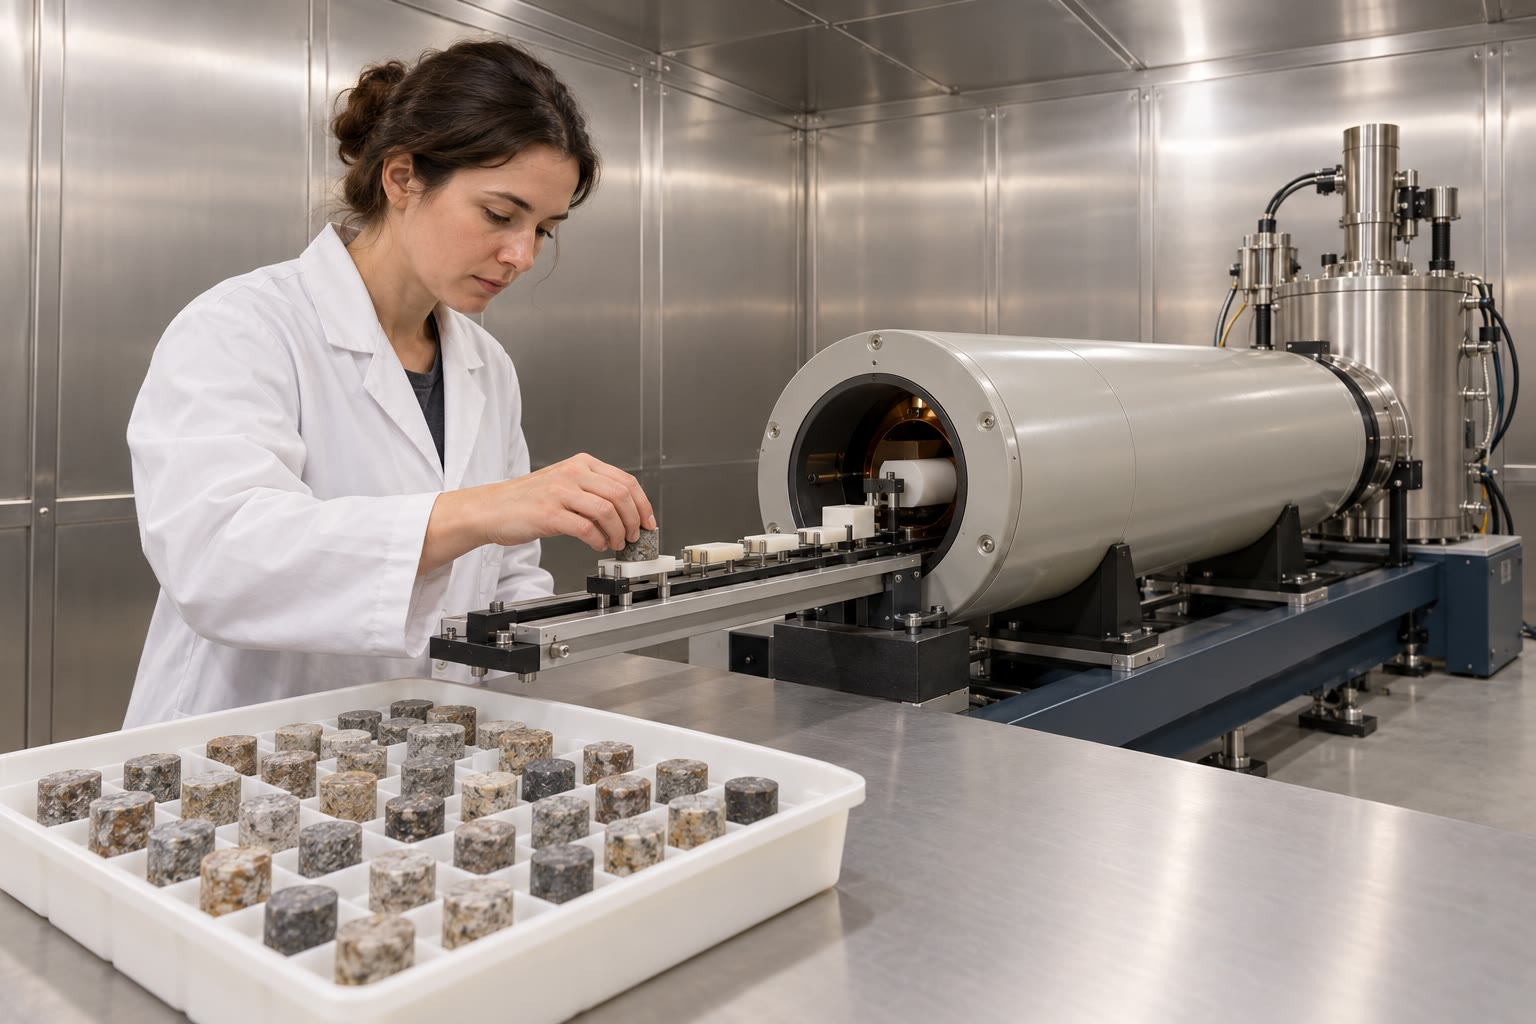
\includegraphics[width=\linewidth]{images/book5/ai/b3-palaeomag-lab.jpg}

{\scriptsize 将样品装上磁力计的样品托盘，该磁力计位于
屏蔽室内（AI 生成插图）。}
\end{minipage}
\end{inthelab}

\section{练习}

\begin{exercise}[$\star$]\label{exo:b3:palaeomagnetism:1}
在\omterm{def:b3:palaeomagnetism:main-field}{地心轴向偶极子}场中，求纬度
北纬 \ang{30} 处的倾角，以及倾角为 \ang{-20} 的测点的纬度。
\end{exercise}

\begin{exercise}[$\star$]\label{exo:b3:palaeomagnetism:2}
测点处的磁场分量为 $X = \qty{20000}{nT}$，$Y =
\qty{-2000}{nT}$ 和 $Z = \qty{40000}{nT}$。求 $H$、$F$、
磁偏角和倾角。
\end{exercise}

\begin{exercise}[$\star$]\label{exo:b3:palaeomagnetism:3}
2025 年，$g_1^0 = \qty{-29350}{nT}$。将磁场视为轴向偶极子场，
求赤道和两极处的磁场强度，以及偶极矩
（$a = \qty{6371.2}{km}$，$\mu_0 = 4\pi\times\qty{e-7}{H.m^{-1}}$）。
\end{exercise}

\begin{exercise}[$\star$]\label{exo:b3:palaeomagnetism:4}
说出所获剩磁的类型，以及它何时记录了地磁场：
（a）熔岩流冷却；（b）粉砂在安静的湖泊中沉降；（c）砂岩中的
氧化铁包膜在早期埋藏时转变为赤铁矿；（d）玄武岩在现今磁场中
静置一百万年。
\end{exercise}

\begin{exercise}[$\star\star$]\label{exo:b3:palaeomagnetism:5}
某测点的四个样品给出方向 $(D, I)$：$(\ang{12}, \ang{48})$，
$(\ang{22}, \ang{44})$，$(\ang{16}, \ang{57})$ 和 $(\ang{6}, \ang{53})$。
求各自的单位矢量、合矢量长度 $R$、平均方向、$k$
和 $\alpha_{95}$。
\end{exercise}

\begin{exercise}[$\star\star$]\label{exo:b3:palaeomagnetism:6}
某测点位于北纬 \ang{40.0}、东经 \ang{10.0}，其平均方向为 $D = \ang{20}$，
$I = \ang{50}$。求该点的\omterm{def:b3:palaeomagnetism:vgp}{古纬度}及其\omterm{def:b3:palaeomagnetism:vgp}{虚地磁极}。
\end{exercise}

\begin{exercise}[$\star\star$]\label{exo:b3:palaeomagnetism:7}
\omterm{def:b3:palaeomagnetism:igrf}{国际地磁参考场}给出，1900 年偶极矩为 \qty{8.32e22}{A.m^2}，
2025 年为 \qty{7.69e22}{A.m^2}；$g_1^0$ 的变化率为
\qty{+12.6}{nT/\text{年}}（2025 年）。（a）求偶极矩每
世纪的相对变化。（b）若 $g_1^0$ 保持该变化率，经过多少年它将变为零？
这为何不是预测？
\end{exercise}

\begin{exercise}[$\star\star$]\label{exo:b3:palaeomagnetism:8}
某样品的剩余剩磁以 \unit{mA/m}（北、东、下）表示，
加热至 \qty{20}{\celsius} 后为 $(32.2, 18.1, 38.2)$，加热至
\qty{300}{\celsius} 后为 $(25.8, 18.1, 24.6)$，加热至 \qty{580}{\celsius} 后为 $(0.0, 0.0, 0.0)$；每两步之间
的正交矢量图均为直线。求 20 至 \qty{300}{\celsius} 之间去除的分量
及 \qty{300}{\celsius} 以上去除的分量的方向和强度。
哪一个是\omterm{def:b3:palaeomagnetism:zijderveld}{特征剩磁}（ChRM），另一个
是什么？
\end{exercise}

\begin{exercise}[$\star\star$]\label{exo:b3:palaeomagnetism:9}
某地层给出 $I = \ang{-35}$，$\alpha_{95} = \ang{5}$。求其
\omterm{def:b3:palaeomagnetism:vgp}{古纬度}，由 $I \pm \alpha_{95}$ 所允许的\omterm{def:b3:palaeomagnetism:vgp}{古纬度}范围，
以及其极点的置信椭圆的半轴 $\mathrm dp$ 和
$\mathrm dm$。
\end{exercise}

\begin{exercise}[$\star\star\star$]\label{exo:b3:palaeomagnetism:10}
(a) 由\cref{thm:b3:palaeomagnetism:dipole}，求\omterm{def:b3:palaeomagnetism:inclination}{磁倾角}为
\ang{45} 的纬度，以及两极处磁场与赤道处磁场之比。
(b) 证明 $\mathrm dI/\mathrm d\lambda = 2/(1 + 3\sin^2\lambda)$，
由此推出倾角误差在何处会使\omterm{def:b3:palaeomagnetism:vgp}{古纬度}误差最大。
(c) 为什么由低倾角得到的\omterm{def:b3:palaeomagnetism:vgp}{古纬度}，
以度计时最为精确？
\end{exercise}

\begin{exercise}[$\star\star\star$]\label{exo:b3:palaeomagnetism:11}
某地点位于一稳定板块上，坐标为南纬 \ang{35.0}、东经 \ang{150.0}，
该板块的参考极点（对应此处所采地层的年龄）位于北纬 \ang{70.0}、
东经 \ang{300.0}。(a) 求该地点到极点的角距离 $p$，
预期的倾角与偏角，以及预期的\omterm{def:b3:palaeomagnetism:vgp}{古纬度}。
(b) 该地层给出 $D_o = \ang{30.0}$，$I_o = \ang{-60.0}$。计算
旋转 $R$ 与向极位移 $P$，并说明其含义。
\end{exercise}

\begin{exercise}[$\star\star\star$]\label{exo:b3:palaeomagnetism:12}
(a) 由\cref{prop:b3:palaeomagnetism:fisher}，证明一方向与均值方向的夹角
不超过 $\theta$ 的概率为 $(e^\kappa -
e^{\kappa\cos\theta})/(e^\kappa - e^{-\kappa})$。(b) 当 $\kappa$ 很大、
$\theta$ 很小时，证明此式约等于 $1 - e^{-\kappa\theta^2/2}$，
由此推出约 \qty{63}{\percent} 的方向落在 $\theta_{63} \approx
\ang{81}/\sqrt\kappa$ 的范围内。(c) 计算 $\theta_{63}$，设 $\kappa = 50$，
并用精确公式检验 \qty{63}{\percent}。
\end{exercise}

\section{问题：凯斯塔红层}

\begin{problem}[{周末问题——一个位移地体的三套地层，
它们的方向、极点与旋转，以及最年轻地层的年龄}]
\label{pb:b3:palaeomagnetism:1}
% values: calc/ch04.py; palaeomag_stats.py, magnetostratigraphy.py; GPTS: iodp:gpts2004
凯斯塔是一个虚构的地体，现位于北纬 \ang{47.0}、东经 \ang{15.0}，位于
一个虚构稳定大陆的边缘。该地体出露三套红层：A，
\qty{60}{Ma}；B，\qty{30}{Ma}；C，约自 3.7 至 \qty{2.4}{Ma}。每套地层
均在若干采样点取样，所有样品均经热退磁处理；
\omterm{def:b3:palaeomagnetism:zijderveld}{特征剩磁} ChRM 由赤铁矿携带，各地层均为水平产状。

\medskip\noindent\textbf{第一部分——平均方向。}地层 A 的六个采样点
给出 $(D, I)$：$(\ang{50}, \ang{37})$，$(\ang{28}, \ang{37})$，
$(\ang{21}, \ang{42})$, $(\ang{24}, \ang{27})$, $(\ang{37}, \ang{39})$,
$(\ang{46}, \ang{38})$.
\begin{enumerate}
  \item 为什么红层中由赤铁矿携带的 ChRM 可能比所在岩层
        更年轻？什么证据能说明它并非年轻很多？
  \item 计算第一个方向的单位矢量。
  \item 六个单位矢量之和为 $(3.8943, 2.6500, 3.5717)$。计算 $R$ 及
        地层 A 的平均方向。
  \item 计算地层 A 的 $k$ 与 $\alpha_{95}$。
  \item 地层 B 由 7 个采样点给出 $D = \ang{23.9}$，$I = \ang{51.5}$ 以及
        $R = 6.8979$；地层 C 由 8 个采样点给出 $D = \ang{3.4}$，$I =
        \ang{63.7}$，$R = 7.8707$。计算二者的 $k$ 与 $\alpha_{95}$。
  \item 哪一套地层的方向最为集中？哪一个平均方向最为确定？
\end{enumerate}

\medskip\noindent\textbf{第二部分——\omterm{def:b3:palaeomagnetism:vgp}{古纬度}与极点。}
\begin{enumerate}[resume]
  \item 计算 A、B 与 C 的\omterm{def:b3:palaeomagnetism:vgp}{古纬度}。
  \item 对地层 A，计算古余纬 $p$ 以及
        其\omterm{def:b3:palaeomagnetism:vgp}{虚地磁极}的纬度。
  \item 计算该极点的经度，并检验
        \cref{thm:b3:palaeomagnetism:pole} 中的哪一种情形适用。
  \item 计算 A 的极点的 $\mathrm dp$ 与 $\mathrm dm$。
  \item B 与 C 的极点分别位于北纬 \ang{66.5}、东经 \ang{135.6}，以及
        北纬 \ang{87.1}、东经 \ang{139.1}。请描述三个极点
        随年龄变化的路径。
\end{enumerate}

\medskip\noindent\textbf{第三部分——地层 C 的年龄。}在地层 C 中，
自其底部起，样品在 \qty{4.2}{m} 以下为反极性，
至 \qty{14.8}{m} 为正极性，至 \qty{19.7}{m} 为反极性，至 \qty{24.6}{m} 为正极性，至
\qty{29.2}{m} 为反极性，至 \qty{54.0}{m} 为正极性，然后直至顶部，
\qty{64.0}{m} 处为反极性。在 \qty{22}{m} 处有一火山灰层，其年龄约为 \qty{3.2}{Ma}。
C2An 极性时中的正极性亚时跨越 3.596--3.330、3.207--3.116 与
3.032--\qty{2.581}{Ma}。
\begin{enumerate}[resume]
  \item 利用火山灰层，将各极性带与地磁极性年表对应起来。
  \item 计算第一与第三个反极性界线之间的沉积速率，
        以及第四与第六个界线之间的沉积速率。
  \item 估计该剖面底部与顶部的年龄。
  \item 为什么该速率是数十万年间的平均值，
        以及哪些因素可能使其发生变化？
\end{enumerate}

\medskip\noindent\textbf{第四部分——相对稳定大陆及其漂移。}稳定大陆的
参考极点位于北纬 \ang{78.0}、东经 \ang{190.0}
（$A_{95} = \ang{3.0}$），对应 \qty{60}{Ma}；北纬 \ang{83.5}、东经 \ang{175.0}
（$\ang{2.5}$）对应 \qty{30}{Ma}；以及北纬 \ang{87.5}、东经 \ang{150.0}（$\ang{2.0}$）
对应 \qty{4}{Ma}。
\begin{enumerate}[resume]
  \item 计算凯斯塔到 \qty{60}{Ma} 参考极点的角距离，
        并计算预期的倾角与\omterm{def:b3:palaeomagnetism:vgp}{古纬度}。
  \item 计算 \qty{60}{Ma} 时的预期偏角。
  \item 在 30 与 \qty{4}{Ma} 时的预期方向分别为 $(\ang{2.9},
        \ang{60.0})$ 与 $(\ang{2.5}, \ang{63.6})$。计算
        A、B 与 C 的向极位移 $P$。
  \item 计算 A、B 与 C 的旋转 $R$。
  \item 计算 A 的误差 $\Delta D_o$ 与 $\Delta D_x$，以及
        其旋转的误差。
  \item B 与 C 的 $R$ 误差分别为 \ang{13.8} 与 \ang{17.9}。哪些
        旋转在 \qty{95}{\percent} 的置信水平上显著？
  \item 叙述凯斯塔相对稳定大陆的运动历史。
  \item 计算自地层 A 形成以来凯斯塔向北的漂移量，相对于自转轴，
        以度和千米为单位
        （每度 \qty{111.19}{km}）。
  \item 计算地层 A 由 $I \pm \alpha_{95}$ 所允许的\omterm{def:b3:palaeomagnetism:vgp}{古纬度}，
        并取该区间宽度之半除以
        1.96 作为一个标准差，给出凯斯塔自地层 A 形成以来向北的漂移量
        （以千米计）及其标准差。
\end{enumerate}
\end{problem}
